\section{Convolutional Neural Networks}
\begin{itemize}
	\item Images are stationary signals with spatial structure and huge dimensionality
	\item Input dimensions are highly correlated (e.g. translation invariant)
	\item Preserve spatial structure by convolutional filters, local connectivity (with shared weights) and being robust to local variances by spatial pooling
\end{itemize}
\subsection{Transfer Learning}
\begin{itemize}
	\item Use large datasets like ImageNet to learn useful features for other, smaller datasets
	\item Prevent overfitting, even for large networks
	\item Alternatively, we could also use a pre-trained network on task 1 as feature extractor for task 2 (same as freezing first layers)
	\item Which layer(s) to fine-tune?
	\begin{itemize}
		\item If both task have the same labels, we can initialize all layers. Otherwise, the classification layer (last layer) must be newly trained. If there is only very few data available, only fine-tune this layer
		\item If datasets are very different, the fully connected layers need to be replaced
		\item First convolutional filters capture low-level information that mostly does not change over datasets. Mid-level convolutions can be fine-tuned if dataset is large enough
	\end{itemize}
	\item Use a smaller learning rate for pre-initialized layers as network starts already from a point close to the optimum. New layers can be trained with higher learning rate
\end{itemize}
\subsection{Standard classification architectures}
\subsubsection{VGGNet}
\begin{itemize}
	\item All filter sizes are $3\times 3$, as this is the smallest filter size, and is more parameter efficient to build up large filters, plus additional non-linearity between filters
	\item $1\times 1$ convolutions used to increase non-linearity/complexity without increasing receptive field
\end{itemize}
\begin{figure}[ht!]
	\centering
	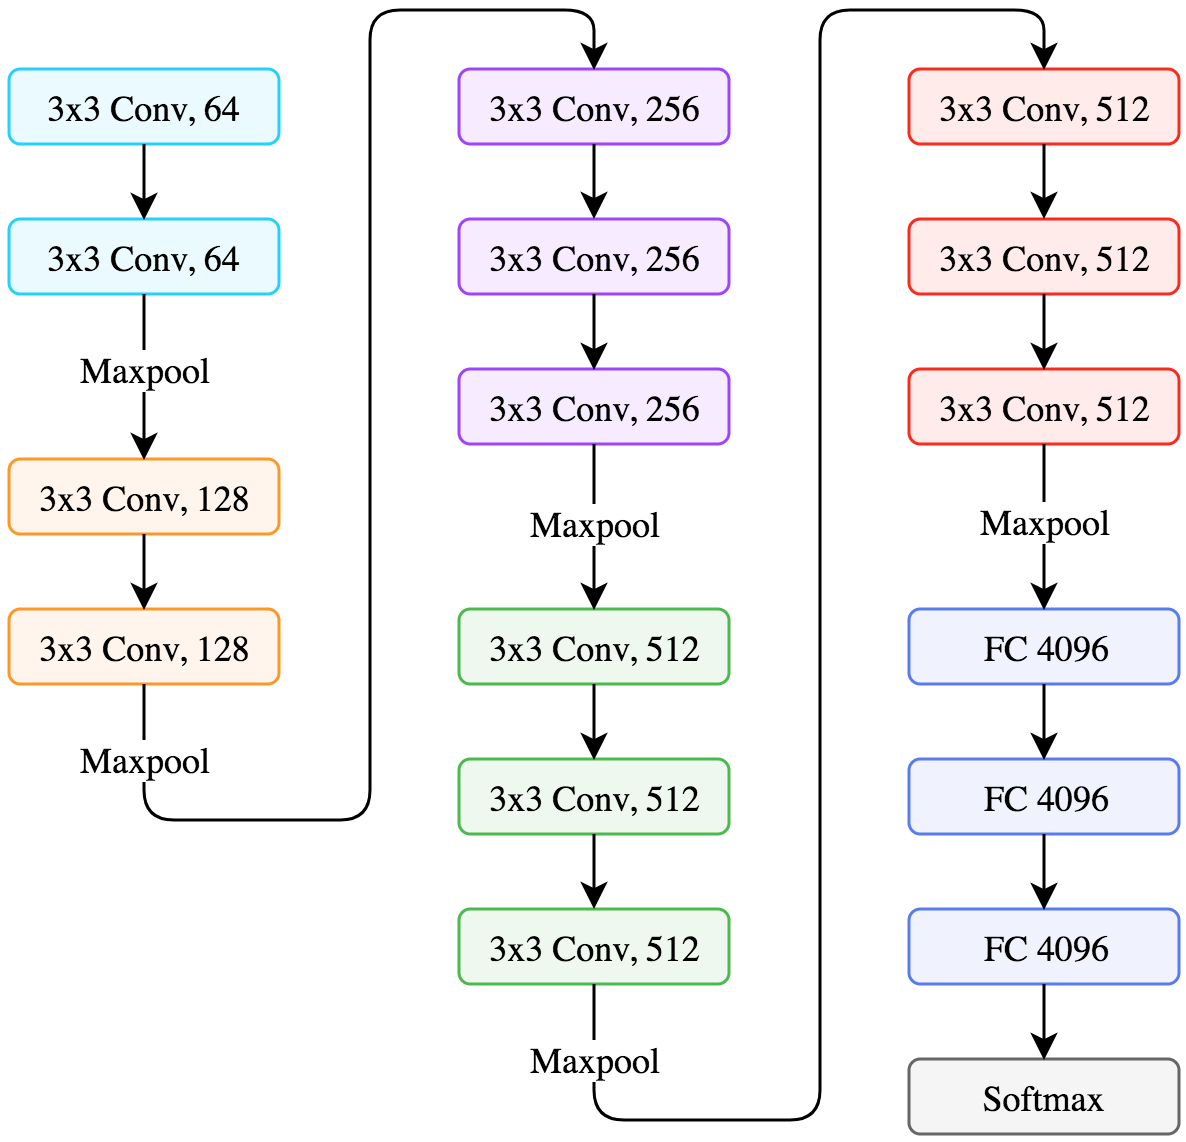
\includegraphics[width=0.3\textwidth]{figures/CNN_VGGnet.png}
	\caption{VGG16 architecture}
	\label{fig:CNN_VVGnet}
\end{figure}
\subsubsection{Inception}
\begin{itemize}
	\item Receptive fields should vary in size as objects can appear in different scales
	\item Naively stacking more convolutional operations on top of each other is expensive and prone to overfitting
	\item Inception module applies different filter sizes on same input ($1\times 1$ convolutions for feature reduction)
	\item Architecture consists of 9 Inception blocks
	\item Solution for vanishing gradients: have intermediate classifiers that amplify the gradient signal for early layers
	\item InceptionV2: $5\times 5$ replaced by two $3\times 3$ filters
	\item InceptionV3: $1\times 3$ and $3\times 1$ filters instead of $3\times 3$
	\item BatchNormalization has shown to be very helpful in this architecture
\end{itemize}
\begin{figure}[ht!]
	\centering
	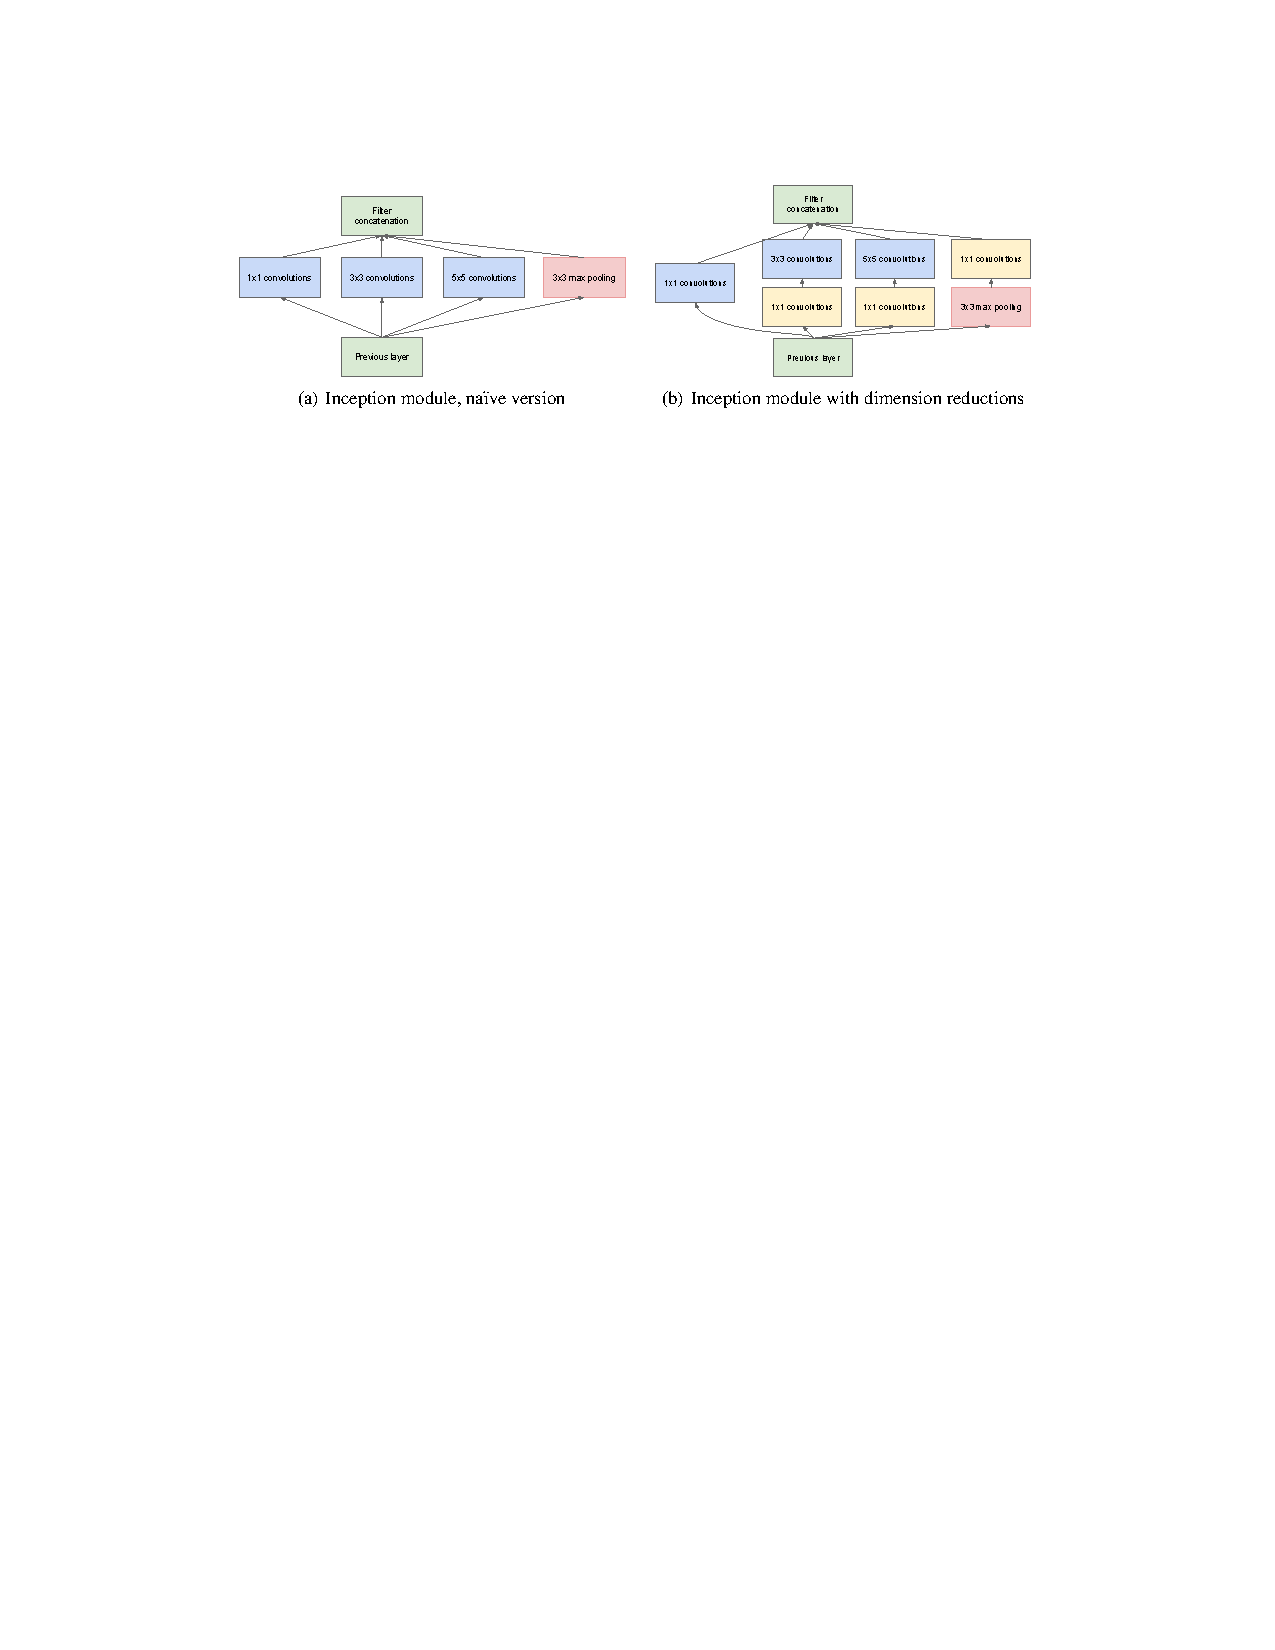
\includegraphics[width=0.8\textwidth]{figures/CNN_Inception_module.pdf}
	\caption{Inception module}
	\label{fig:CNN_Inception_module}
\end{figure}
\subsubsection{ResNet/DenseNet/HighwayNet}
\begin{itemize}
	\item Deeper networks are harder to optimize, and might actually achieve worse results than shallow ones because of that (although learning identity in additional layers must lead to same results)
	\item Better approach: try to model the difference that is learned in every layer $H(x) = F(x) + x$
	\item Different ways for modeling $F(x)$. Most popular ones shown in Figure~\ref{fig:CNN_ResNet_blocks}. BatchNormalization has been shown to be very important because of vanishing gradients
	\begin{figure}[ht!]
		\centering
		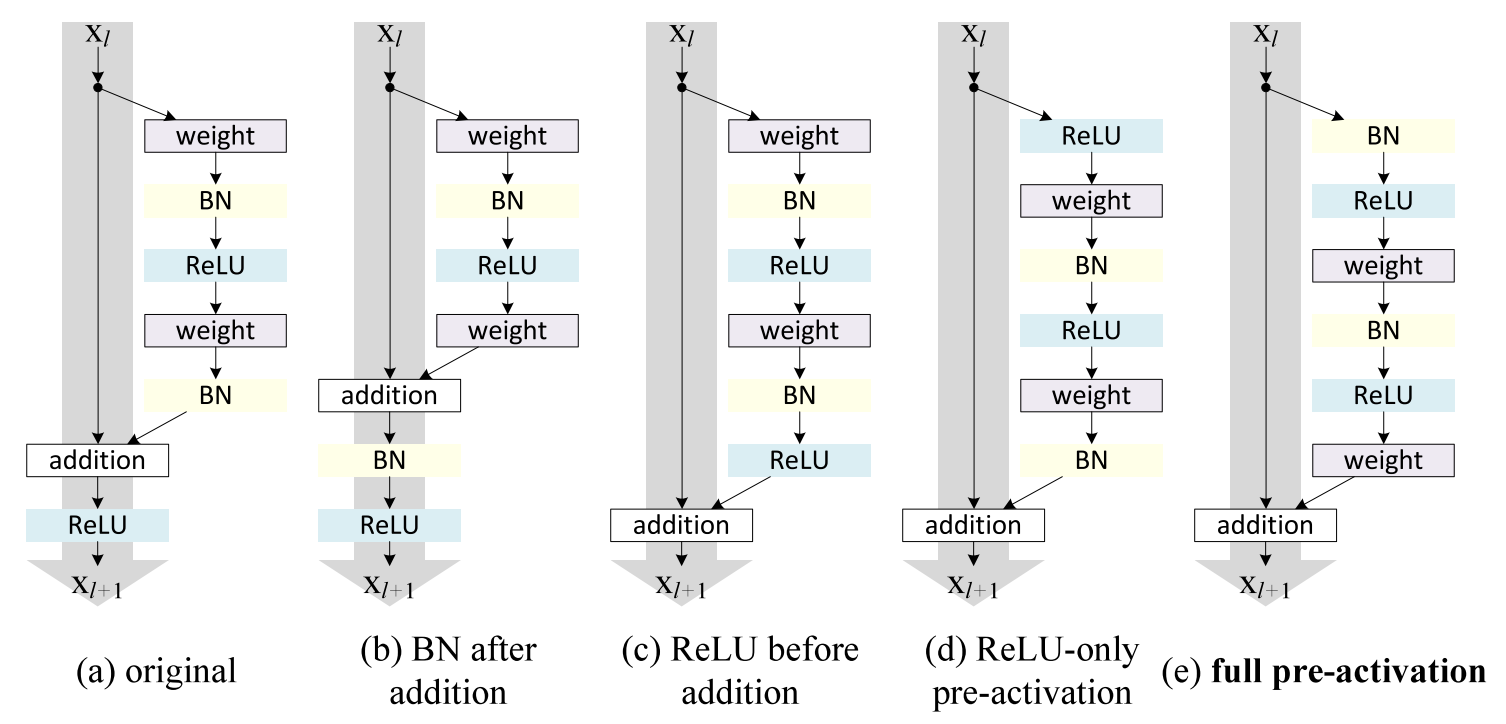
\includegraphics[width=0.7\textwidth]{figures/CNN_ResNet_blocks.png}
		\caption{ResNet blocks}
		\label{fig:CNN_ResNet_blocks}
	\end{figure}
	\item \textbf{HighwayNet} introduces a gate with learnable parameters to determine the importance of a layer: $H(x) = F(x) \cdot T(x) + x \cdot \left(1 - T\left(x\right)\right)$
	\item \textbf{DenseNet} uses skip connections to multiple forward layers. Creates complex blocks where last layer sees the input of all previous layers
\end{itemize}
\subsection{Tracking/Object detection}
\subsubsection{Fast R-CNN}
\begin{itemize}
	\item Based on middle feature map, get bounding boxes by e.g. selective search 
	\item RoI pooling returns fixed size feature map for selected bounding box (puts e.g. $3\times 3$ mask on features and pools accordingly)
	\item Features used to generate class prediction and location correction
	\item During training, sample multiple candidate boxes from image and train on all of them. Makes it more efficient/faster, \textit{but} batch elements might be highly correlated (in the paper, they report that they experienced it to be neglectable)
	\item Very accurate and fast, but external box proposals needed
	\item \textbf{Faster R-CNN}: train network to propose box locations
\end{itemize}
\subsubsection{Siamese Network for Training}
\begin{itemize}
	\item Use Siamese network to compare similarity of two patches
	\item If we compare patches over time, we can find objects with the highest similarity $\Rightarrow$ tracking of objects
	\item Can be trained on rich video dataset, and can be applied to unseen categories/targets
\end{itemize}
\subsection{Spatial Transformer Network}
\begin{itemize}
	\item ConvNets must be invariant/robust to pose/geometry changes. One simple way of doing it is data augmentation
	\item Better: use spatial transformer network to learn rotation/scale transformation
	\item Define grid on input. Scale, translation and rotation parameters are learned by the network and depend on the input. Finally, transform image based on the changed grid. 
	\item Operation is differentiable and thus can be learned
\end{itemize}